\documentclass{article}
\usepackage{xecjk}
\usepackage{graphicx}

\title{Computer Architecture Lab1 Report}
\author{PB17111568 郭雨轩}
\date{\today}
\begin{document}
    \maketitle
    % \begin{figure}[htbp]
    %     \includegraphics[scale=0.07]{figures/CA.pdf}
    % \end{figure}
    \section{前言}
    \paragraph{}
    由于本实验仓库中提供的数据通路参考图内容存在错误且部分项目不全,
    故本实验和下一个实验基于的数据通路是我在提供的图上补充了一点细节后形成的,我的数据通路会以附件的形式上交。
    我使用的数据通路中 所有的控制信号如下:
    \begin{figure}[htbp]
        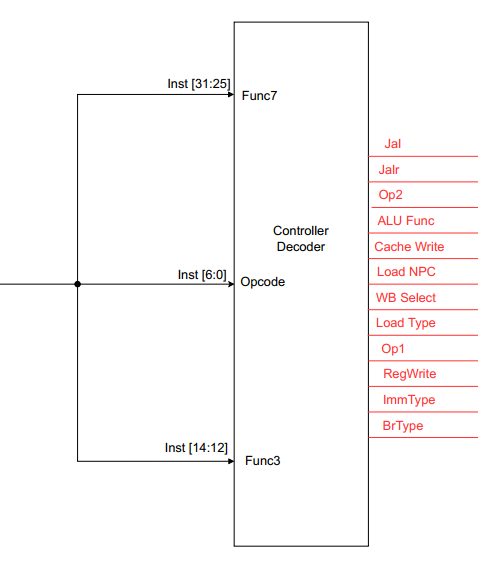
\includegraphics[scale=0.5]{figures/1.png}
    \end{figure}
    
    \section{实验报告}
    \subsection{描述执行一条 ADDI 指令的过程(数据通路、控制信号等)}
    \paragraph{}
    控制信号:Op1选通寄存器值,Op2选通立即数Imm,
    ALUFunc立即数加法,ImmType表明为I-type的立即数,WBSelect选通ALU输出,RegWrite有效,LoadNPC选择ALU输出,其余信号全部无效。
    

    数据通路:首先得到rs1和imm的值,进入ex段经ALU计算得到结果,经过两个选择器后写回寄存器。
    \subsection{描述执行一条 JALR 指令的过程·(数据通路、控制信号等)}
    \paragraph{}
    控制信号:Jalr有效,Op选通寄存器,Op2选通立即数Imm,ALUFunc加法,LoadNPC选通PC+4,ImmType为I-type,
    RegWrite有效,WBselect选通ALU结果,其余信号无效。
    

    数据通路:首先得到rs1和imm的值,进入ex段经ALU计算得到跳转的目的地址,写回PC;另一方面,PC+4的结果经过两个数据选择器写回寄存器。

    \subsection{描述执行一条 LW 指令的过程(数据通路、控制信号等)}
    \paragraph{}
    控制信号:Op1选通寄存器值,Op2选通立即数Imm,ALUFunc加法,LoadNPC选通ALU,WBSelect选择cache数据,
    LoadType为lw,RegWrite有效,ImmType为I-type。
    

    数据通路:首先得到rs1和imm的值,进入ex段经ALU计算得到结果,作为地址去cache中读数据,然后经过LoadType的数据扩展后,写回寄存器。
    \subsection{如果要实现 CSR 指令(csrrw,csrrs,csrrc,csrrwi,csrrsi,csrrci),设计图中还需要增
    加什么部件和数据通路?给出详细说明}
    \begin{itemize}
        \item IF:无
        \item ID:完善立即数扩展模块,加入CSR扩展的格式支持;添加CSR寄存器文件;控制单元需要额外生成CSR读写使能信号;将符号扩展后的CSR送入ID/EX段寄存器;
        \item EX:在Op2数据选择器处加入CSR;ALU运算结果送入EX/MEM
        \item MEM:运算结果送入MEM/WB
        \item 写回通用寄存器和CSR
    \end{itemize}
    \subsection{哪些指令分别采用了五类立即数(I-type,S-type,B-type,U-type,J-type 至少各举
    一例)?Verilog 如何将这些立即数拓展成 32 位的}
    \begin{itemize}
        \item ADDI, I-Type: $sext(inst[31:20])$
        \item SW, S-Type: $sext(inst[31:25] || inst[11:7])$
        \item BEQ, B-Type: $sext(inst[31]||inst[7]||inst[30:25]||inst[11:8])$
        \item AUIPC, U-Type: $sext(inst[31:12]<<12)$
        \item JAL, J-Type: $sext(inst[31:12])$
    \end{itemize}
    \subsection{如何实现 Data Cache 的非字对齐的 Load 和 Store}
    \paragraph{}
    在cache内部使用字节交叉编址,按照地址mod4的余数将不同的字节映射到4个不同的存储体,根据load和store指令格式,选择相应的存储体进行存储。
    \subsection{ALU 模块中,默认 wire 变量是有符号数还是无符号数}
    \paragraph{}
    无符号。
    \subsection{哪条指令执行过程中会使得 Load Npc == 1}
    \paragraph{}
    Jal, Jalr
    \subsection{NPC Generator 中对于不同跳转 target 的选择有没有优先级}
    branch, Jalr > Jal (EX段指令优先,因为不考虑乱序的情况下,EX段指令靠前)
    \subsection{Harzard 模块中,有哪几类冲突需要插入气泡}
    \begin{itemize}
        \item Load-Use型
        \item 分支和跳转
    \end{itemize}
    \subsection{Harzard 模块中采用默认不跳转的策略,遇到 branch 指令时,如何控制 flush 和 stall 信
    号}
    \begin{itemize}
        \item branch ID
        \item branch IF 下一条指令IF
        \item branch EX 下一条指令ID,下下条指令IF,此时branch是否跳转已经确定,若不跳转则不需要flush和stall;
        否则Flush IF/ID和ID/EX.
    \end{itemize}
    \subsection{0 号寄存器值始终为 0,是否会对 forward 的处理产生影响}
    \paragraph{}
    需要在实现转发控制信号的时候对源寄存器是x0的情况进行特殊判断(组成原理课本有提及),当某条运算指令写的是x0寄存器时,不能对后续指令转发运算结果,而是需要转发0。
\end{document}